\documentclass[a4paper, 11pt, oneside]{article}

\usepackage[utf8]{inputenc}
\usepackage[T1]{fontenc}
\usepackage[english]{babel}
\usepackage{array}
\usepackage{shortvrb}
\usepackage{listings}
\usepackage[fleqn]{amsmath}
\usepackage{amsfonts}
\usepackage{fullpage}
\usepackage{enumerate}
\usepackage{graphicx}
\usepackage{alltt}
\usepackage{indentfirst}
\usepackage{eurosym}
\usepackage{titlesec, blindtext, color}
\usepackage[table,xcdraw,dvipsnames]{xcolor}
\usepackage[unicode]{hyperref}
\usepackage{url}
\usepackage{float}
\usepackage{subcaption}
\usepackage[skip=1ex]{caption}
\usepackage{dsfont}

\definecolor{brightpink}{rgb}{1.0, 0.0, 0.5}

\usepackage{titling}
\renewcommand\maketitlehooka{\null\mbox{}\vfill}
\renewcommand\maketitlehookd{\vfill\null}

\newcommand{\ClassName}{INFO8011: Network Infrastructures}
\newcommand{\ProjectName}{Software-Defined Networking in Data Centers}
\newcommand{\AcademicYear}{2021 - 2022}

%%%% First page settings %%%%

\title{\ClassName\\\vspace*{0.8cm}\ProjectName\vspace{1cm}}
\author{Maxime Goffart \\180521 \and Olivier Joris\\182113}
\date{\vspace{1cm}Academic year \AcademicYear}

\begin{document}

%%% First page %%%
\begin{titlingpage}
{\let\newpage\relax\maketitle}
\end{titlingpage}

\thispagestyle{empty}
\newpage

%%%%%%%%%%%%%%%%%%%%%%%%%%%%%%%%%%%%%%%%%%

\section{General overview}

\subsection{Spanning Tree Controller}
\paragraph{}This controller, as requested, builds a spanning tree in order to handle cycles in the network. To implement this solution, we first needed to discover the topology of the network. To do so, we used the functions \texttt{get\_host}, \texttt{get\_link}, and \texttt{get\_switch} of Ryu.\\
Then, based on the discovered topology, we built a graph of the topology where the vertices are the switches and the edges are the links between the switches. Afterwards, to compute the minimal spanning tree, we used Prim's algorithm.\\
\indent When packets are received at the controller, through \texttt{switch\_in\_handler} method, we check the source and the destination of each packet.\\
If the source is one of the host and the destination is broadcast, we broadcast the packet to the switches connected to the one that received it in the minimal spanning tree. Thus, the switches to which we sent the packet will send the packet to the controller that will, once again, do the same processing. At the same time, we set flows in the different switches so the controller will be contacted only once for a particular type of packets and it will reduce the RTT for similar requests.\\
If the source and the destination are both hosts, we compute a path between them using a depth-first search algorithm. Of course, the path is limited to links in the minimal spanning tree. When the path is computed, we set flows in the switches along the path so the controller will be contacted only once for a particular type of packets and it will reduce the RTT for similar request.

\subsection{Adaptive routing} \label{subsec:adaptive}
\paragraph{}Unfortunately, we were not able to implement this controller. The reason is that we are supposed to use \texttt{OFPPortStatsRequest}, but, when we listen for the response, \texttt{EventOFPPortStatsReply}, in an handler, the reponse is always empty. Here is a screenshot of the execution of the code on one of our machine:
\begin{figure}[H]
\centering
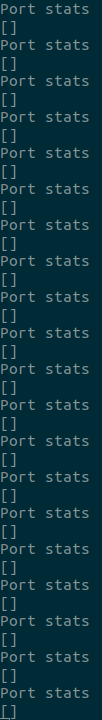
\includegraphics[scale=0.3]{port_stats.png}
\end{figure}
Thus, the file \texttt{adaptive.py} is just a copy of \texttt{spanningtree.py} with the code to handle \texttt{OFPPortStatsRequest} that always provides an empty response.

%%%%%%%%%%%%%%%%%%%%%%%%%%%%%%%%%%%%%%%%%%

\section{Tests}

\subsection{Spanning Tree Controller}
\subsubsection{Tests in normal conditions}
\paragraph{}If we ping 10 times each host from \texttt{h0}, we obtained the results of table \ref{table:STCPings}. The simple commands used are available in the file \texttt{test\_spanning\_tree.sh}.\\
\begin{table}[]
\centering
\begin{tabular}{|l|l|l|l|}
\hline
\multicolumn{1}{|c|}{\textbf{Source-Dest}} & \multicolumn{1}{c|}{\textbf{Mean}} & \multicolumn{1}{c|}{\textbf{MDEV}} & \multicolumn{1}{c|}{\textbf{1st ping}} \\ \hline
H1-H2                                      & 272ms                              & 201ms                              & 877ms                                 \\ \hline
H1-H3                                      & 466ms                              & 124ms                              & 840ms                                 \\ \hline
H1-H4                                      & 460ms                              & 124ms                              & 830ms                                 \\ \hline
H1-H5                                      & 695ms                              & 192ms                              & 1274ms                                 \\ \hline
H1-H6                                      & 693ms                              & 188ms                              & 1258ms                                 \\ \hline
H1-H7                                      & 691ms                              & 208ms                              & 1317ms                                 \\ \hline
H1-H8                                      & 707ms                              & 198ms                              & 1300ms                                 \\ \hline
H1-H9                                      & 715ms                              & 210ms                              & 1347ms                                 \\ \hline
H1-H10                                      & 707ms                              & 200ms                              & 1306ms                                 \\ \hline
H1-H11                                     & 703ms                              & 200ms                              & 1300ms                                 \\ \hline
H1-H12                                     & 678ms                              & 192ms                              & 1256ms                                 \\ \hline
H1-H13                                     & 705ms                              & 181ms                              & 1247ms                                 \\ \hline
H1-H14                                     & 640ms                              & 15ms                              & 649ms                                 \\ \hline
H1-H15                                     & 694ms                              & 197ms                              & 1287ms                                 \\ \hline
H1-H16                                     & 701ms                              & 200ms                              & 1302ms                                 \\ \hline
\end{tabular}
\caption{Results of 10 pings between each host and \texttt{h0}}
\label{table:STCPings}
\end{table}
We can see that the first ping always take a lot of time. This is explained because the first ping we will have as consequence to send multiple packets to the controller. First, it will send packets to the controller related to the ARP request to learn the MAC address of the destination. Then, it will send packets to the controller related to the icmp messages which will require the computation of paths between the host and the destination. All the processing in the controller is done in Python which is well known to be a slow language. Furthermore, these tests were performed on Maxime's computer which had the vm lock with an execution cap at 10\% (see in section \ref{sec:feedback} the explanation).\\
Yet, the pings, after the first one of each test, have a RTT around the mean value. The high values of MDEV are explained by the fact that the first ping take a lot of time thus it increases the values of MDEV.\\
Another reason for the high value is the fact that each link has a delay of 50ms as set in the Mininet topology provided. Finally, we should keep in mind that we are running in a virtual environment and not on physical devices thus the measurements are not the most precise. Also, real physical links would not have a delay of 50ms (except for very long distance).
tree[i][0] == None or tree[i][1] == None
\subsubsection{Tests when a switch/link fails}
\paragraph{}First, we can try to ping \texttt{h5} from \texttt{h1} and \texttt{h15} from \texttt{h1}. Both pings work as expected. Now, let us simulate a switch failure by typing \texttt{switch s17 stop} in Mininet. Then, ping \texttt{h5} from \texttt{h1} and \texttt{h15} from \texttt{h1}. Both work because our controller react to the change of topology. Now, let us simulate the switch going back up by typing \texttt{switch s17 start} in Mininet and do the same 2 pings as before. Both work because our controller react to the change of topology.\\
This simple test is available in the file \texttt{test\_spanning\_tree\_failure.sh}.

\subsection{Adaptive routing}
\paragraph{}As explained in section \ref{subsec:adaptive}, we were not able to implement this controller. Thus, there is nothing to test.

%%%%%%%%%%%%%%%%%%%%%%%%%%%%%%%%%%%%%%%%%%

\section{Feedback} \label{sec:feedback}
\subsection{Main difficulties}
\paragraph{}We encountered multiple difficulties when working on this assignment. Here is a list of the difficulties we encountered:
\begin{itemize}
\item Instabilities of the virtual machine, Mininet, and Ryu. For instance, Maxime had to cap the execution of the processor for the virtual machine at 10\% or the code would not work. He lost some time trying to understand the issue. An other example is what we experienced in section \ref{subsec:adaptive}.
\item Most documentations, even the official book, on how to use Ryu is for OpenFlow 1.3 while we were blocked to OpenFlow 1.0. The differences between the 2 versions are minors but they are resulting in lose time that could be used to improve our understanding of SDN. Also regarding documentations, they are not always very well done.
\end{itemize}
These difficulties have the consequence that we have the impression that we spent more time on details related to Ryu and different versions of OpenFlow than really improving our understanding of SDN. Furthermore, these difficulties increased the difficulty of the project uselessly.

\subsection{Time spent on the project}
\paragraph{}Unfortunately, Maxime did not keep track of the time he spent on the project.

\subsection{Possible improvements}
\paragraph{}Here is a list of possible improvements for the project:
\begin{itemize}
\item Switching to OpenFlow 1.3 because, as mentioned previously, most documentations on Ryu are using OpenFlow 1.3 and we will not lose time on details related to which version of OpenFlow we are using.
\item Maybe using something else than Ryu because we had issues related to it (e.g. needing to cap the execution of the processor or some functions of Ryu would return anything).
\end{itemize}

%%%%%%%%%%%%%%%%%%%%%%%%%%%%%%%%%%%%%%%%%%
\end{document}